\section{Protein biology}
Proteins are an essential part of molecular biology and are involved in almost all cellular functions. They are part of the essential biological macromolecules that make up life, hence a lot of effort has gone towards trying to understand the functions of protein and disruptions in its mechanisms that lead to many kinds of diseases. Proteins are composed of a linear chain of amino acids (AA) with a length ranging from 50 to tens of thousands of AAs, all connected by peptide bonds into a polypeptide. This is also referred to as the \textit{primary structure} of a protein as mentioned earlier~\cite{primstruct}. A sequence of amino acids is mostly determined by the genetic code without considering post-translational and post-transcriptional modifications etc. In the genetic code of all living organisms, there are 20 different kinds of amino acids coded in that make up the `language' of proteins. Each amino acid has the same backbone but differs by the chemical properties of its side chain, also known as the R-group. This sequence of amino acids does not occur as a mere linear chain of peptides and consists of much more intricacies. The protein's \textit{secondary structure} is formed by locally folded structures in the polypeptide chain, excluding the R-group. This folding is caused by chemical interactions within the backbone. The most common and well-known examples of these structures are the $\alpha$-helices and $\beta$-sheets. The overall three-dimensional structure that forms out of these structures is referred to as the \textit{tertiary structure}. These are formed due to interactions between the R-groups and are much harder to classify due to the quasi-infinite amount of potential conformations that could occur in a protein structure~\cite{folding}. And lastly, a protein can also be made up of multiple polypeptide chains, referred to as its subunits. These subunits together form the \textit{quaternary structure} of a protein.

The sought-after biochemical and cellular functions of a protein emerge from a combination of all of these structures. While a protein's 3D structure and function are dynamic and dependent on its surroundings such as the cellular state and other proteins and molecules, it is still defined by its underlying sequence. This means that a lot of the 3D-structural and functional information of a protein should be retrievable from its amino acid sequence~\cite{structure}. Understanding how a protein's sequence translates to its structure and function, otherwise known as the `protein folding problem', is the central problem of protein biology and is crucial for understanding disease mechanisms and designing proteins and drugs for therapeutic and bioengineering applications. Therefore, a lot of effort has gone into computational methods for structure and function predictions from protein sequences but this sequence-structure-function relationship continues to challenge bioinformaticians. In the remainder of this chapter, we will discuss state-of-the-art bioinformatics methods to obtain more knowledge in this field.

\section{Computational approaches to understand protein biology}
\subsection*{State-of-the-art approaches}
As mentioned earlier, the Edman degradation method was mostly used before to determine the primary structure of a protein. The current state-of-the-art methods for the identification of protein sequences are \textit{de novo sequencing} algorithms applied to tandem mass spectrometry data~\cite{protseq} and allow simultaneous sequencing of thousands of proteins per given sample. Plenty of valuable biological and evolutionary information is already retrievable from just the primary structure \textit{via} traditional tools such as BLAST and MSA as discussed earlier and could provide more information for the prediction of secondary and tertiary structures. However, to cope with the number of recorded protein sequences rising exponentially, far more compute-efficient methods based on multiple sequence alignments had to be developed like PSI-BLAST~\cite{psiblast}, HHblits~\cite{hhblits3} and MMseqs~\cite{mmseqs2}. However, it's important to note that these methods might struggle to handle the continuously growing number of protein sequences stored in databases. As illustrated in Figure~\ref{fig:pdb}b, the UniProt Archive (UniParc) has seen a significant increase in recorded protein sequences, with the count now exceeding half a billion.

\begin{figure}[!ht]
    \centering
    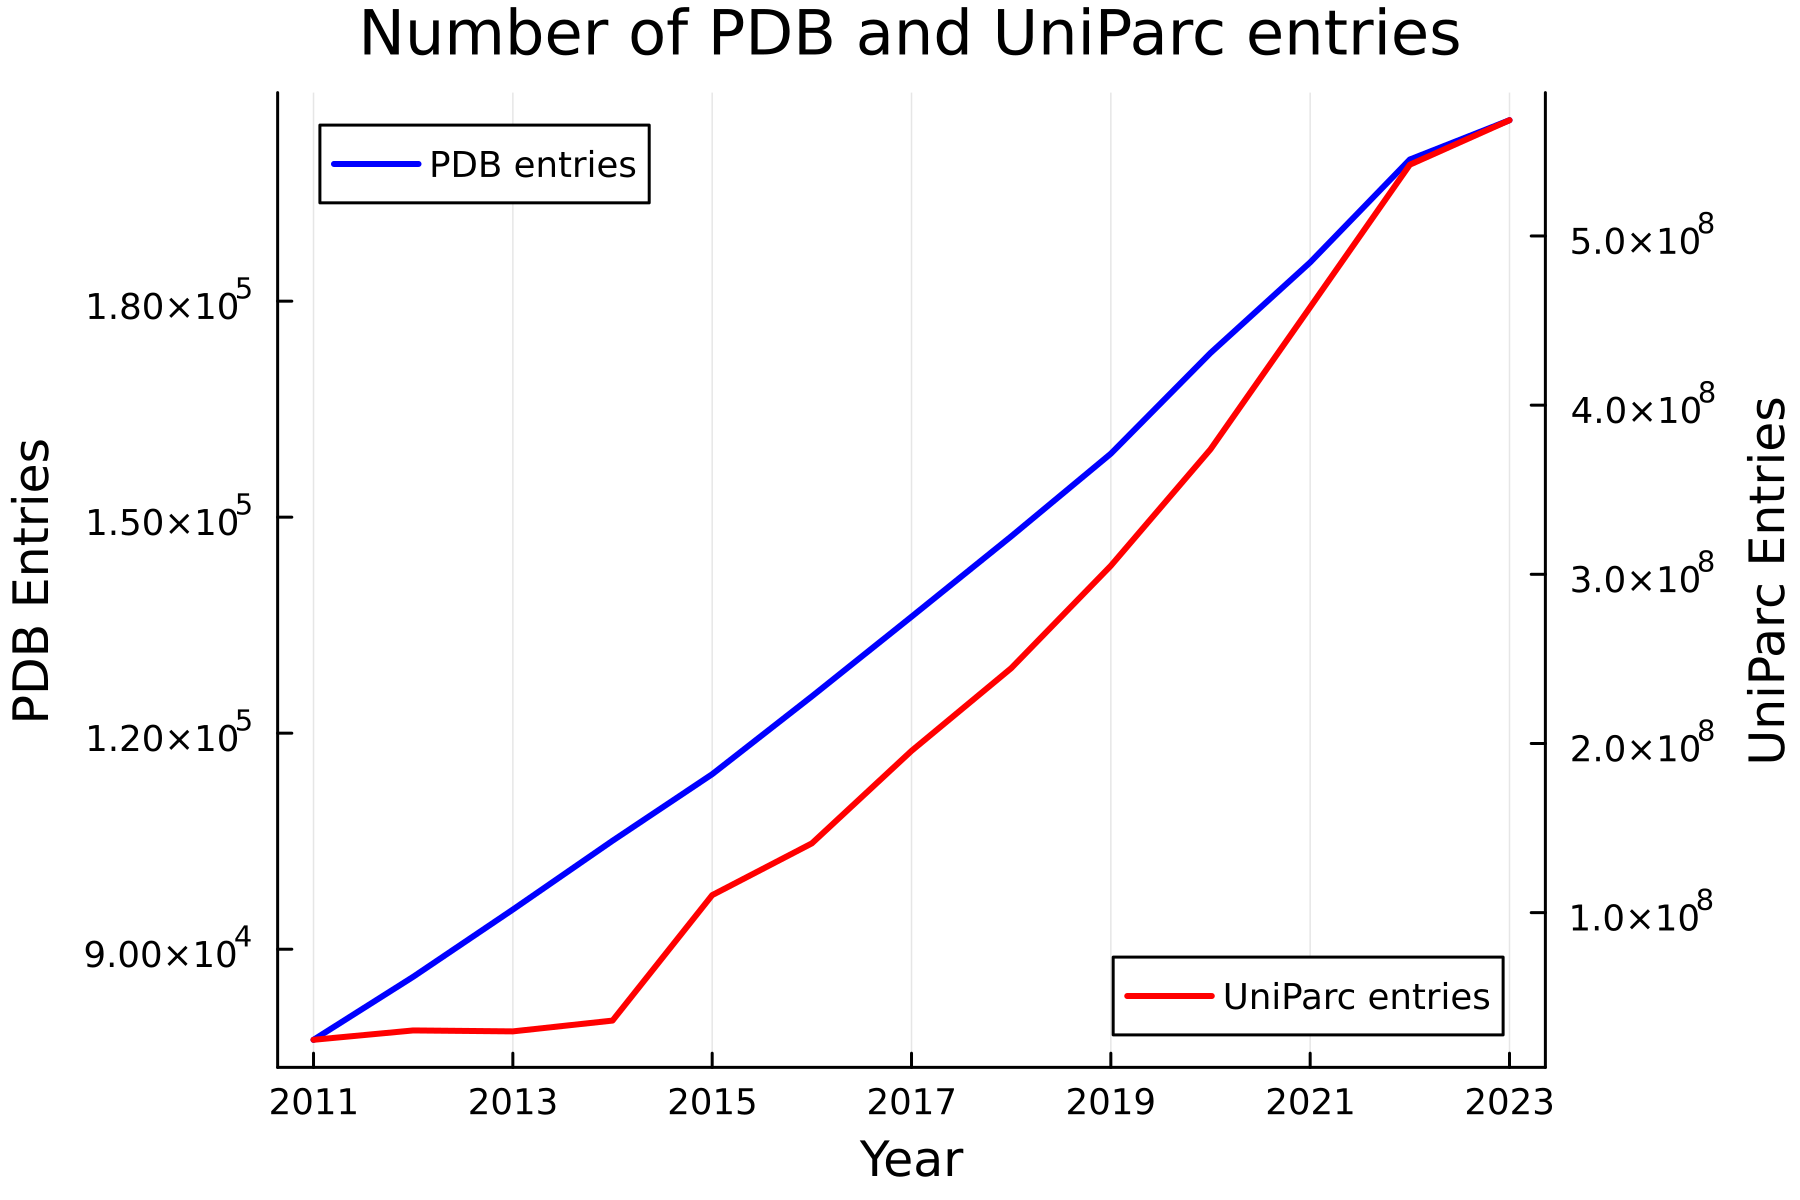
\includegraphics[scale = 0.25]{combined_plot_lines.png}
    \caption{Total number of entries in PDB~\cite{pdb} in blue and the total number of entries in UniParc~\cite{uniprot} in red, from 2011 to 2023 as of May 2023. Note the different scales.}
    \label{fig:pdb}
\end{figure}

At the other end of the spectrum, the most common way to determine the 3D structure of a protein has remained to be X-ray crystallography for more than half a century~\cite{xray}, with cyro-electron microscopy now catching up rapidly~\cite{cyroem}. However, these kinds of laboratory approaches for structure determination of proteins are complex, expensive and in some cases not possible for the protein in question whilst sequence determination is relatively much easier to perform. Because of that, the structures and functions for a large fraction of the approximately 20000 known human proteins remain unknown~\cite{coverage}. When we look at Figure~\ref{fig:pdb} and compare the number of entries in the Protein Data Bank (PDB)\cite{pdb} - a key database for protein structures - with the number of protein sequences in the UniProt Archive (UniParc)~\cite{uniprot}, it becomes clear that the growth of the number of verified three-dimensional structures in protein databases is not keeping up with the rapid increase in sequence information. This growing gap highlights the increasing importance of computational models that can predict protein structure and function.

A lot of methods have been developed to tackle this problem. Until recently, these methods were mainly based on statistical sequence models or physics-based structural simulations. \textit{Ab initio} physics-based approaches such as ROSETTA~\cite{rosetta} solve this problem by searching the protein's conformational space using atom energy functions and minimizing the total free energy of the system. ROSETTA has shown to be effective at predicting unknown structures and has been widely used for varying applications, but also assumes simplified energy models, is extremely computationally intensive and has limited accuracies~\cite{review}. Statistical sequence modeling of a set of related proteins, on the other hand, has proven to be very useful for discovering evolutionary constraints, homology searches and predicting residue-residue contacts. Improvement of these models has mainly been data-driven; exploiting databases to build large deep learning systems which culminated in the recent success of DeepMind's AlphaFold2~\cite{alphafold2} at the Critical Assessment of Protein Structure Prediction (CASP) 14. This success of AlphaFold continued into more recently CASP 15~\cite{casp15}. Even though, DeepMind did not participate, the most successful participants integrated AlphaFold into their methods. However, all of these models are supervised methods that require labels. Labeled protein structure data essentially means retrieving the 3D coordinates of every atom in a protein which is very labor-intensive and time-consuming. Also, such kind of models would likely perform poorly when working with completely unrelated proteins since the model won't be trained on this kind of data. 

One underlying theme of these computational methods for protein structure prediction is being able to translate the protein `language' into numerical representations which computers can learn from. This is now known as the field of protein language modeling.

\subsection*{Protein language modeling}\label{ssec:nlp}
It is intuitive to represent a protein as a sequence of letters with each letter corresponding to an amino acid. As with natural languages, we can find common elements between naturally evolved proteins. Noticeable patterns reoccurring in multiple (related) protein sequences are highly likely to be biologically relevant. These motifs and domains are essential to many biological processes and can easily be represented as words, phrases or sentences of amino acids in a language model perspective. This is why researchers are taking inspiration from the recent successes of natural language processing (NLP) and applying this to a biological context. NLP is a branch of artificial intelligence (AI) concerning itself with creating the ability for computers to learn and understand (human) languages by using statistical, machine learning and in recent years deep learning models~\cite{Ofer}. Common tasks in NLP include part-of-speech tagging (grouping words based on their function in a sentence), named entity recognition (recognizing specific entities in a sentence such as locations, persons, dates etc.) and natural language generation (letter/word prediction).

As with protein language modeling, applying labels to millions of natural language data such as web pages, articles, journals etc. is a labor-intensive procedure and thus state-of-the-art NLP models use a form of \textit{self-supervised learning}, a form of unsupervised learning in which the context of the text is learned to fill in missing words, predict the next word in a sentence etc. during the training as shown in Figure~\ref{fig:ofer}. This masked learning paradigm involves tokenizing input text into smaller units and converting them into numerical representations, followed by random masking of a certain percentage of tokens in the input sequence. The masked input sequence is then fed through multiple layers of a neural network architecture, which capture different levels of semantic and syntactic information, resulting in contextualized embeddings~\cite{esm}. Finally, the model can be fine-tuned on a specific task using supervised learning. Through self-supervised masked learning, language models can learn a wide range of linguistic patterns and structures, enabling them to generate meaningful text, answer questions etc. The principles of self-supervised learning and masked learning from NLP can be adapted to the "language" of proteins to learn how a protein sequence translates to a three-dimensional structure~\cite{review}.

\begin{figure}[!ht]
    \centering
    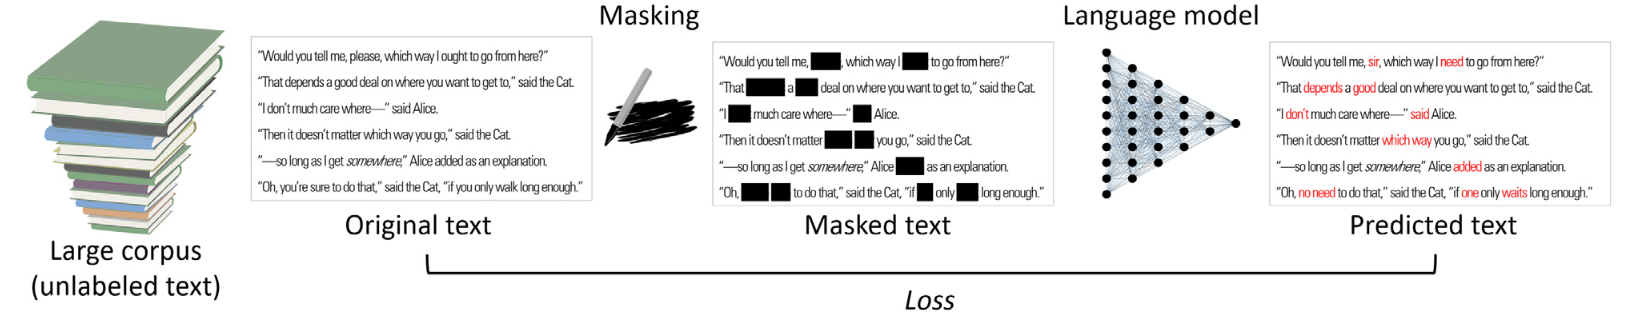
\includegraphics[scale = 0.375]{ofer_cropped.png}
    \caption{Demonstration of a self-supervised masked language learning model. A fraction of the unlabeled text is masked randomly and the language model will attempt to predict these masked tokens. The loss function is a method to assess the performance of the model on its predictions}
    \label{fig:ofer}
\end{figure}

Well-known NLP methods which adapt some kind of self-supervision include bi-directional long-short term recurrent neural networks (biLSTMs) such as ELMo~\cite{elmo} and more recently transformers such as Google's BERT~\cite{bert} and OpenAI's GPT-3~\cite{gpt3} and GPT-4~\cite{gpt4}. Despite the simplicity of the idea behind self-supervision, such models pre-trained at scale have shown interesting capabilities with very little training on a specific task, now mostly referred to as \textit{few-shot learning}~\cite{review}. 

In recent years, transformers have become the backbone of many state-of-the-art NLP and protein language models. Transformers are a class of neural network architectures that have revolutionized the field of natural language processing (NLP) since their introduction by Vaswani \textit{et al.} in 2017~\cite{transfor}. The key innovation of transformers is the self-attention mechanism, which allows the model to weigh the importance of each input token in relation to the others, enabling the efficient handling of long-range dependencies in text. Similar to NLP tasks, protein language models can be pre-trained on large-scale unlabeled protein sequence databases, to learn general features of protein sequences in an unsupervised manner. These pre-trained models can then be fine-tuned on specific protein-related tasks with limited labeled data.

State-of-the-art protein models leverage other advanced machine learning techniques to capture complex patterns in amino acid sequences and predict protein properties. These models employ a combination of sequence alignments, evolutionary information, and NLP-inspired transformer-based architectures to achieve remarkable performance in predicting protein structures and function with the most notable latest projects being TAPE~\cite{tape}, ProtTrans~\cite{prottrans} and Meta AI's ESM-2~\cite{esm2}, one of the most recent and largest protein language models to ever have been developed at the time of writing. ESM-2 has been shown to accurately capture evolutionary information and to perform well on structure prediction tasks. It consists of transformer-based protein language models with up to 15 billion parameters trained on 65 million unique sequences.

As with natural language models, a consistent trend has been observed in protein language models wherein increasing the number of parameters and the amount of training data leads to ever-increasing performance. Remarkably, performance does not appear to saturate even with the largest models~\cite{Ofer}. However, the computational power required to train such models and perform predictions with them grows exponentially with the number of parameters, reaching a point where modern computers struggle to keep up in a sustainable manner. For instance, training the 175 billion parameter GPT-3 model with 300 billion tokens is estimated to take at least 34 days using 1024 NVIDIA A100 GPUs~\cite{gptrain}. While these advancements in computational modeling are undeniably impressive, they come with significant environmental costs in terms of energy consumption and material resources required to support such systems. While the specifics of the infrastructural requirements behind large-scale protein and natural language models, including applications like OpenAI's ChatGPT, aren't typically made publicly accessible, we can still make some educated guesses about their environmental impact. For instance, it's estimated that the carbon emissions produced during the training process of GPT-3, the model underlying ChatGPT, amounts to 552 tonnes of CO\textsubscript{2}~\cite{co2}. To put this into perspective, it is equivalent to the yearly carbon footprint of nearly 60 average Belgian residents~\cite{ghg}. Even with the vast computational requirements and their consequential environmental impact, it is important to not lose sight of our wider responsibilities in the realm of scientific research. As researchers continue to research natural language processing and protein language modeling, it is crucial to balance the pursuit of ever-larger models with the objective of sustainable and responsible development.